\documentclass[10pt]{article}

% Default 
\usepackage{graphicx}
\usepackage[backend=biber,
  style=numeric, 
  sorting=none]{biblatex}

% Additional
\usepackage{amsmath}
\usepackage{textcomp, gensymb}
\usepackage{placeins}
\usepackage{tabularray} 
\usepackage{xcolor}
\usepackage{placeins}
\usepackage{csquotes} 
\usepackage{todonotes} 
\usepackage{hyperref}

\newcommand{\td}[1]{\todo[linecolor=blue, backgroundcolor=blue!25,bordercolor=blue, size=\small, inline]{#1}}

\addbibresource{references.bib}

\title{Grating Spectrometer} 
\author{Rahmanyaz Annyyev, Hikmat Gulaliyev}
\date{27 April 2024} 

\begin{document}

\maketitle

\begin{abstract}

In this experiment, a grating spectrometer, an optical device similar to a prism that separates light into its constituent wavelengths, was used to measure the spectral lines of a Mercury gas discharge lamp. A collimator with a slit produces a parallel beam of light, that falls on the grating which consists of a large number of evenly and nearly placed narrow slits. As the light passes through the grating, it is diffracted in multiple directions, producing a pattern of bright and dark spots. The bright spots correspond to constructive interference, while the dark spots correspond to destructive interference. The angle of diffraction depends on the wavelength of the light and the spacing of the grating. The light is then focused by a telescope, and the spectral lines are observed. The angle of rotation of the grating is measured for each spectral line, and the wavelength of the light is calculated. Results show that the calculated wavelengths are in good agreement with the literature values.

\end{abstract}

\section{Introduction}

\subsection*{General}

One of the most common devices in optical spectroscopy is the grating spectrometer. The grating spectrometer is an instrument comprised of reflecting or transmitting elements separated by a distance comparable to the wavelength of light under consideration. It is akin to a prism spectrometer except that it uses a grating instead of a prism and produces a higher resolution. Some examples of gratings include a pattern of transparent slits (or apertures) in an opaque screen or a collection of grooves on a substrate. The main purpose of the grating spectrometer is to disperse light into its constituent wavelengths \cite{Palmer_2020}. Parameters that define the grating include the width of the slits, the spacing between the slits, and the total number of slits. Upon incidence, the light is diffracted in multiple directions. The angle of diffraction depends on the wavelength of the light and the spacing of the grating. After diffraction, the light waves interfere with each other, producing a pattern of bright and dark spots. The bright spots correspond to constructive interference, while the dark spots correspond to destructive interference. 

To find the percentage error between the calculated and literature values of the wavelengths, we use the formula
\begin{equation}
  \text{Percentage error} = \left| \frac{\lambda_{\text{c}} - \lambda_{\text{l}}}{\lambda_{\text{l}}} \right| \times 100 \%
\end{equation}
where $\lambda_{\text{c}}$ is the calculated wavelength and $\lambda_{\text{l}}$ is the literature value of the wavelength.

\subsection*{Equipment}

The experimental setup is comprised of a Mercury gas discharge lamp, a collimator, a transmission grating, a rotating table, and a telescope. It is shown in Figure~(\ref{fig:1}). 

\begin{figure}[hbt!]
  \centering
  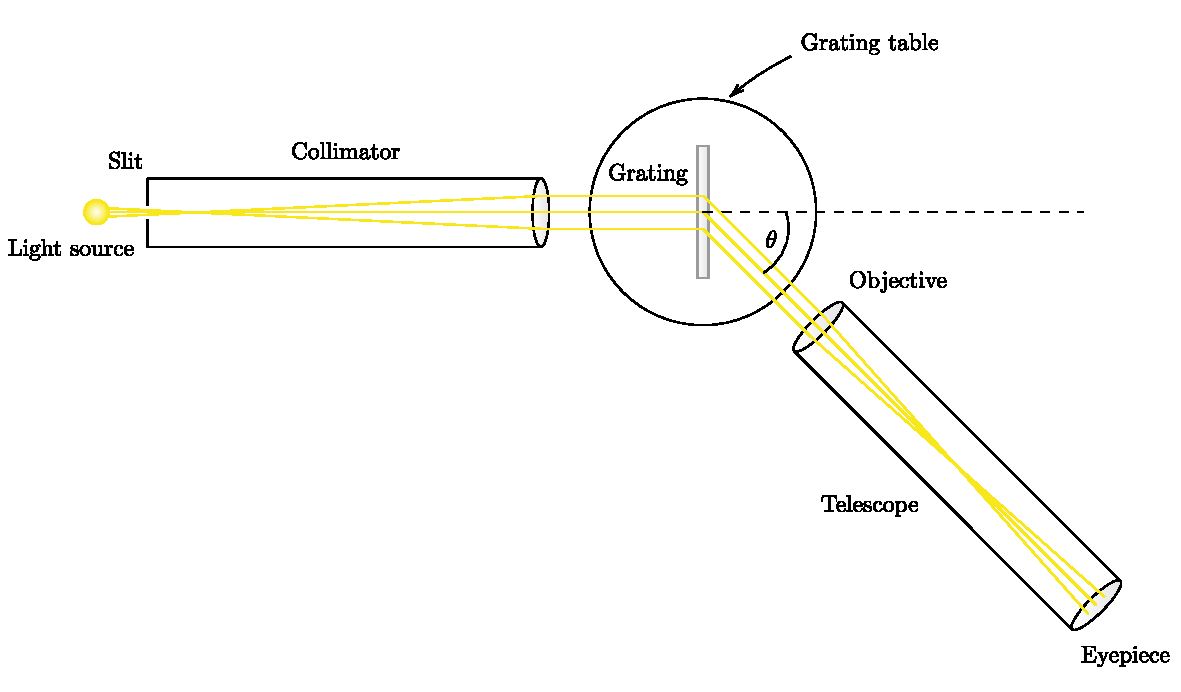
\includegraphics[scale=0.6]{figures/f1.pdf}
  \caption{The experimental setup of the experiment.}
  \label{fig:1}
\end{figure}

\subsection*{Procedure}

First, the Mercury gas discharge lamp is placed in front of the collimator and turned on for ten minutes to allow the lamp to reach a constant temperature. A small rectangle of light should be seen through the collimator. Next, the spectrometer is adjusted so that the collimator produces a parallel beam of light and the telescope receives it in the same way. Then the eyepiece of the telescope is adjusted for optimal focus based on the individual's eyesight. Next, the grating is placed on the rotating grating table and the table is rotated until the first-order spectrum is seen. The height of the table is adjusted so that the full width of the collimated beam is incident on the grating without any blockage. The telescope is then rotated until the first-order spectrum is seen. 

Next, the table is rotated until the plane of the grating is perpendicular to the collimated beam, ensuring the ruled lines face the telescope. When looking through the telescope, a sharp image of the slit should be seen in the center of the field of view (this is the zero-order spectrum). Then, rotate the table to determine the number of visible orders. Realign the telescope arm of the spectrometer with the collimator arm. The image of the slit should be seen once again in the center of the field of view. Next, the cross-hair should be aligned with the center of the slit and the angle of rotation should be recorded. If the zero order is not observed precisely at $0\degree$, the subsequent measurements should be corrected by the same amount.

The telescope should be rotated slowly until a series of spectral lines are seen. The angle of rotation should be recorded for each color. Finally, the process should be repeated for the opposite direction of rotation.

\section{Data \& Results}

\td{!!!}

The results of the experiment are shown in Table~(\ref{tab:1}). The wavelength of light was calculated using the Equation ..., and the percentage error was calculated using the Equation ... 

\begin{table}[ht]
  \centering
  \vspace{4mm}
  \footnotesize
  \begin{tblr}{
    cells = {halign = c, valign = m},
    row{odd} = {bg = lightgray!5},
    row{2} = {bg = lightgray!20},
    hlines = {},
    vlines = {},
    cell{1}{1}={c=3}{l},
    cell{1}{4}={c=4}{l}
  }
    Gas discharge lamp = Mercury & & & Grating spacing ($d$) = 600 lines/mm & & & \\
    \hline
    Color & {$\theta \degree$ \\ (Clock. rot.)} & {$\theta \degree$ \\ (Coun.-clock. rot.)} & {$\theta \degree$ \\ (Average)} & {$\lambda$ nm \\ (Calc.)} & {$\lambda$ nm \\ (Lit.)} & {\% \\ error} \\
    \hline 
    Violet & $14\degree 23'$ & $14\degree 30'$ & $14\degree 26'$ & 415.4 & 404.6 & 2.676 \\
    Violet & $14\degree$ & $14\degree 50'$ & $14\degree 25'$ & 415.0 & 407.8 & 1.765 \\
    Blue & $15\degree$ & $15\degree 30'$ & $15\degree 15'$ & 438.4 & 435.8 & 0.595 \\
    Blue-green & $17\degree 2'$ & $17\degree 35'$ & $17\degree 18'$ & 495.6 & 491.6 & 0.814 \\
    Green & $18\degree 20'$ & $18\degree 40'$ & $18\degree 30'$ & 528.8 & 546.1 & 3.169 \\
    Orange & $20\degree'$ & $21\degree 39'$ & $20\degree 49'$ & 592.3 & 577.0 & 2.649 \\
    Orange & $20\degree 10'$ & $21\degree 58'$ & $21\degree 4'$ & 599.1  & 579.1 & 3.454 \\
  \end{tblr}
  \caption{Results of the grating spectrometer experiment.}
  \label{tab:1}
\end{table}

The resolving power of the grating is given by the formula
\begin{equation}
  R = \frac{\lambda}{\Delta \lambda} = mN
  \label{eq:2}
\end{equation}
where $\lambda$ is the wavelength of the light, $\Delta \lambda$ is the spectral resolution, $m$ is the order of the spectrum, and $N$ is the number of lines per unit length of the grating. The spectral resolution is the smallest wavelength difference that can be distinguished by the grating. 

Let's find the resolving power of the grating for the first three spectral lines. Since the grating spacing is $600$ lines/mm, the number of lines per unit length is $N = 600 \times 10^3$ lines/m. The resolving power is calculated in the following way:
\begin{align}
  &R_1 = 1 \times 600 \times 10^3 = 600 \times 10^3 \text{ lines/m} \\
  &R_2 = 2 \times 600 \times 10^3 = 1200 \times 10^3 \text{ lines/m} \\
  &R_3 = 3 \times 600 \times 10^3 = 1800 \times 10^3 \text{ lines/m}
\end{align}

Let's find the spectral resolution our grating can distinguish near the region of $500$ nm. The spectral resolution is for the first three spectral lines is calculated the following way:
\begin{align}
  &\Delta \lambda_1 = \frac{\lambda}{R_1} = \frac{500 \times 10^{-9}}{600 \times 10^3} = 8.33 \times 10^{-13} \text{ m} = 833 \text{ fm} \\
  &\Delta \lambda_2 = \frac{\lambda}{R_2} = \frac{500 \times 10^{-9}}{1200 \times 10^3} = 4.17 \times 10^{-13} \text{ m} = 417 \text{ fm} \\
  &\Delta \lambda_3 = \frac{\lambda}{R_3} = \frac{500 \times 10^{-9}}{1800 \times 10^3} = 2.78 \times 10^{-13} \text{ m} = 278 \text{ fm}
\end{align}

\section{Discussion \& Conclusion}

\subsection*{Errors}

The sources of error in the experiment include calibration error, instrument resolution and imperfection, human error, spectral overlap, and external factors.

\begin{itemize}
  \item \textbf{Calibration error:} The spectrometer may not have been calibrated precisely enough to ensure parallel beams of light. Since the calibration of the spectrometer was done by eye, without the aid of precise instruments, it may have led to systematic errors in the measurements since it relies on the subjective judgment of the observer. Furthermore, the grating may not have been placed on the rotating table precisely enough to ensure that the ruled lines face the telescope, leading to errors in the measurements.
  
  \item \textbf{Instrument resolution and imperfection:} The instrumental resolution of the spectrometer, determined by factors such as the slit width and the optical design, can limit the ability to resolve closely spaced spectral features, leading to errors in peak identification and intensity measurement. Imperfections in the grating, such as scratches or dust, can also affect the diffraction pattern and lead to errors in the measurements. Furthermore, the telescope may have imperfections that affect the reception of light.
  
  \item \textbf{Human error:} The angle of rotation was measured by eye, which may have introduced errors in the measurements. Furthermore, a vernier scale was used to measure the angle of rotation, which may have introduced both parallax and reading errors. 
  
  \item \textbf{Spectral overlap:} The spectral lines may have overlapped, making it difficult to distinguish between them and leading to errors in the measurements. Furthermore, since the spectrum is continuous, it is difficult to determine the exact wavelength of a spectral line, leading to errors in the measurements. This is especially true for lines that are close together, such as the blue and blue-green spectral lines.
  
  \item \textbf{External factors:} External factors such as ambient light, temperature, and humidity can affect the measurements by introducing noise and errors. 
\end{itemize}

\subsection*{Approximations}

The grating spectrometer is an approximation of the ideal spectrometer. The ideal spectrometer would have a perfect grating with no imperfections, a perfect collimator that produces a parallel beam of light, and a perfect telescope that receives the light in the same way. In reality, the grating may have imperfections that affect the diffraction pattern, the collimator may produce a non-parallel beam of light, and the telescope may not receive the light in the same way. These imperfections can lead to errors in the measurements. 

\subsection*{Discrepancies}

The discrepancies between the calculated and literature values of the wavelengths can be attributed to the sources of error mentioned above. The smallest discrepancy was found in the blue spectral line with a percentage error of 0.595\%, and the largest discrepancy was found in the green spectral line with a percentage error of 3.169\%. However, the discrepancies were generally small, indicating that the experiment was successful in measuring the wavelengths of the spectral lines.

\subsection*{Conclusion}

In conclusion, despite the analog nature of the experiment, sources of error and approximations experiment was successful and the calculated wavelengths were in good agreement with the literature values. The grating spectrometer is a powerful tool for measuring the wavelengths of spectral lines and can be used in a wide range of applications.

\section{Extra Credit}

Diffraction grating is a method used in spectroscopy, a measurement technique that studies the interaction between matter and light at different wavelengths.  
spectroscopy can be used from astronomy to biology, and from chemistry to physics. Some of the more interesting uses of spectroscopy include the study of the composition of stars.
Since each element emits light at specific wavelengths or has a unique fingerprint, spectroscopy can be used to determine the composition of stars by analyzing the light they emit. This can provide information about the temperature, density, and composition of stars, as well as their age and distance from Earth \cite{Banerjee_2022}.

\printbibliography

\end{document}